\section{Results}
\label{sec:results}
The results of our efforts in this project, including the metrics of the model itself and an example of its working state, will be outlined in this section. \\

Our own model was initially trained, requiring a significant amount of time and effort. However, a switch was made to a pre-trained model, which presents the following metrics:\\
\begin{figure}[h]
    \centering
    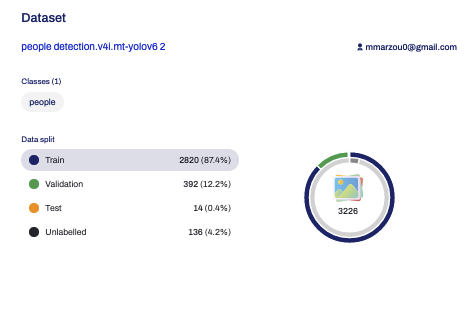
\includegraphics[width=0.5\textwidth]{images/train.png}
    \caption{training data}
    \label{fig:data}
\end{figure}

Our aim was to make our demo publicly available for everyone to test. Azure was utilized to host our solution and the below QR code was created that could be easily scanned, directing users straight to the tool. \\
\begin{figure}[h]
    \centering
    
\includegraphics[width=0.3\textwidth]{images/QR.jpeg}
    \caption{QR code for Demo}
    \label{fig:data}
\end{figure}

Upon arriving at our site, two buttons will be visible: one for uploading a single image and another for uploading three or more images. In this workflow, the complete functionality is demonstrated by selecting more than three images. This selection involves pre-processing to stitch the images together, ensuring uniform size and zoom across all images. The stitching process was performed using the OpenCV Library.\\
\begin{figure}[h]
    \centering
    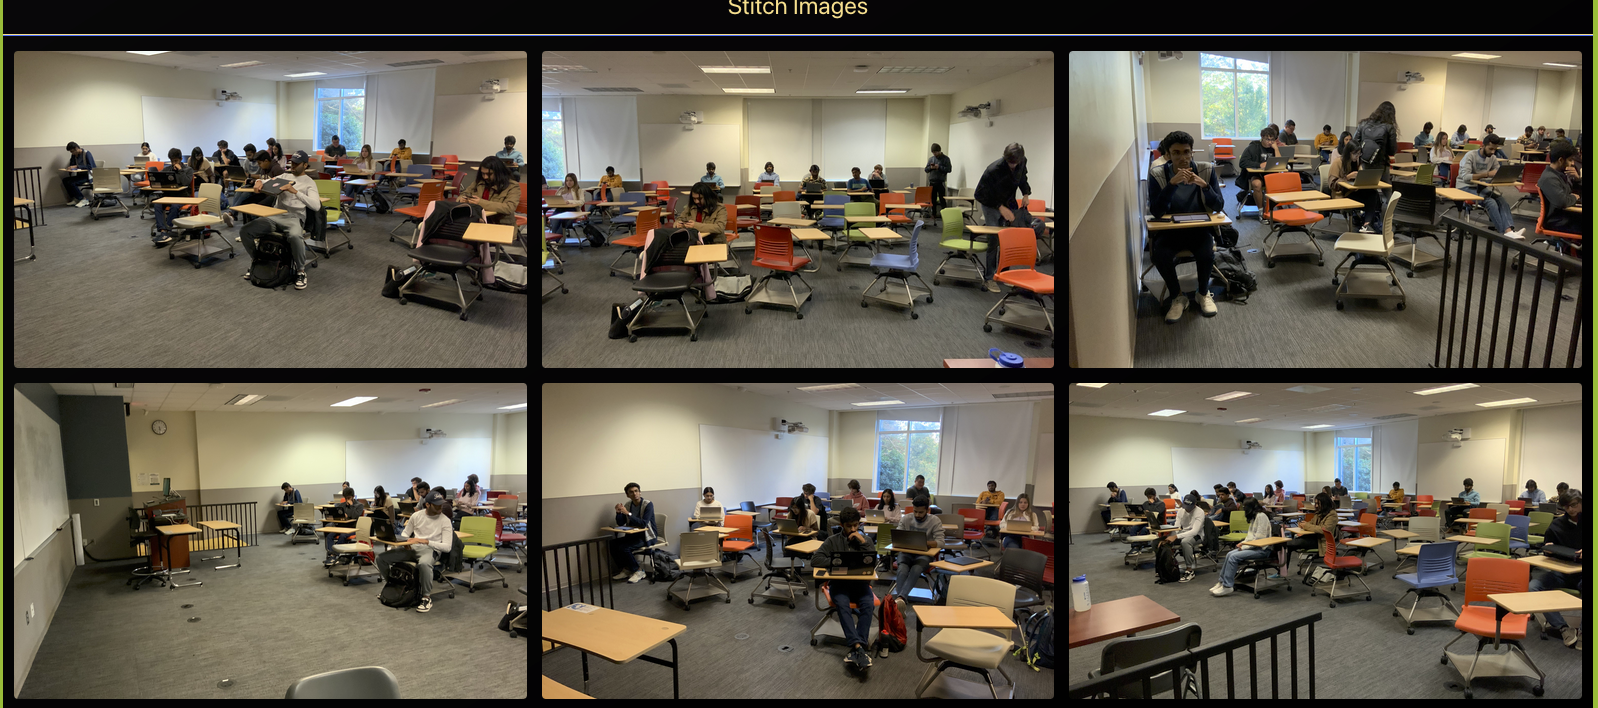
\includegraphics[width=0.5\textwidth]{images/Pre.png}
    \caption{Pre-Processed Image}
    \label{fig:before}
\end{figure}

The figure below shows the image before it is fed into the model after performing the preprocessing and stitching. \\
\begin{figure}[h]
    \centering
    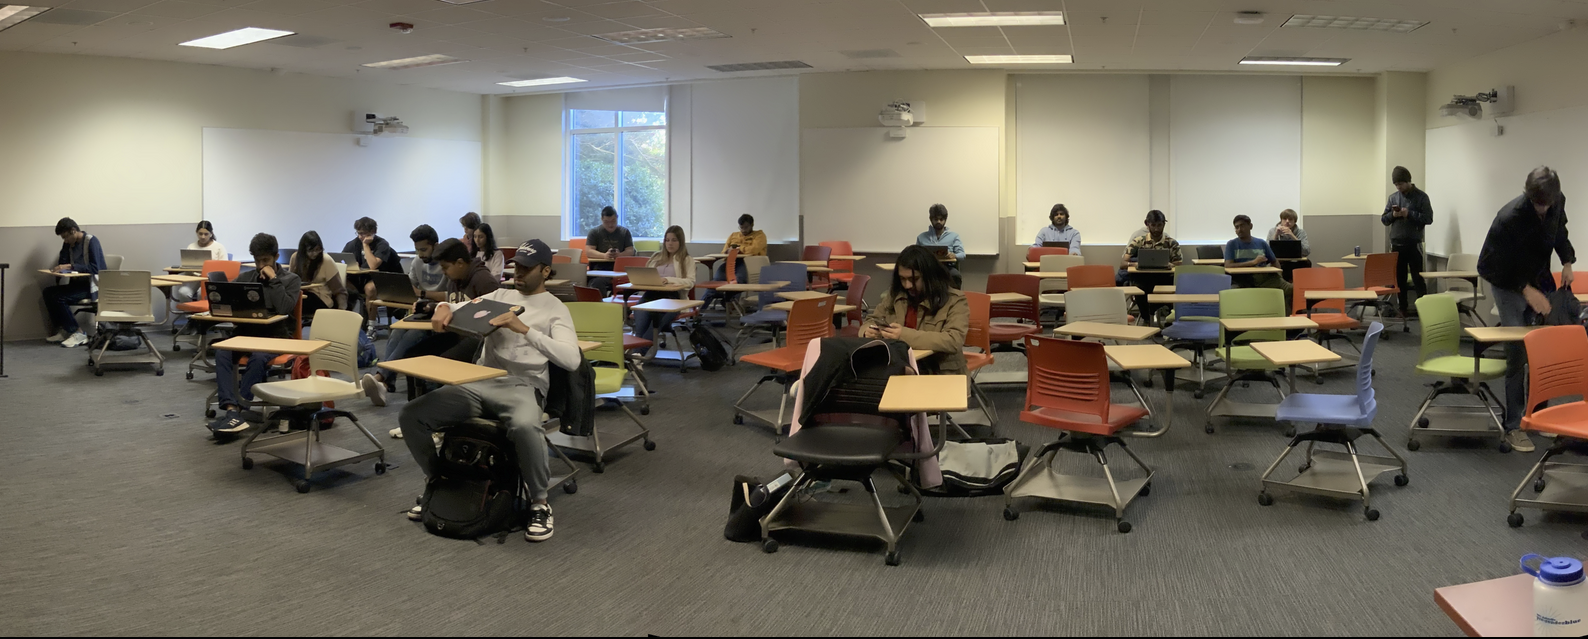
\includegraphics[width=0.5\textwidth]{images/Before.png}
    \caption{Before}
    \label{fig:before}
\end{figure}

The image below shows the results of the model. The model was trained for 100 epochs and the loss was 0.0001. The model that was used was pre-trained on yolov6-n variant of the YOLO family. \\
\begin{figure}[h]
    \centering
    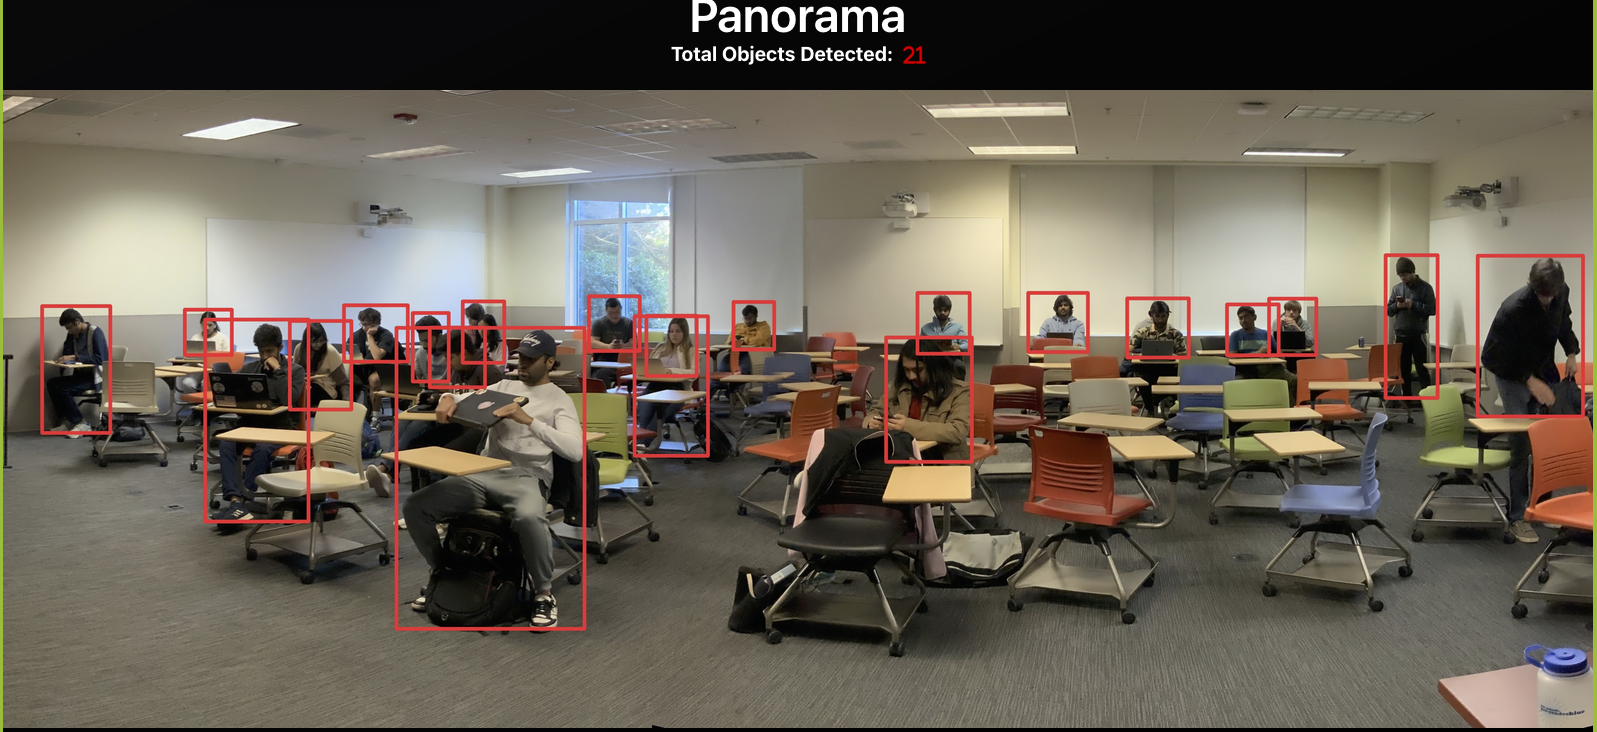
\includegraphics[width=0.5\textwidth]{images/After.png}
    \caption{After}
    \label{fig:after}
\end{figure}

There were 21 total students found in this classroom.
%-------------------------------------------------------------------------
